\section{User Manual}
\label{ss:user-manual}

\subsection{Mobile Client(Android)}
\subsubsection{Getting started and Installation}
To get started download and install the latest version of WiFi mapper from the website provided or from google play app store. If downloaded from the app store, the app will automatically install on your device. If downloaded from the website, tap on the apk file to begin installation. During installation WiFi mapper will ask for permissions to  use location services of the device. Tap yes to allow the app to send data from your device. Tapping no will allow one to see the data collected by other users but will not allow the app to send the data to the database.
\begin{figure}
	\centering
	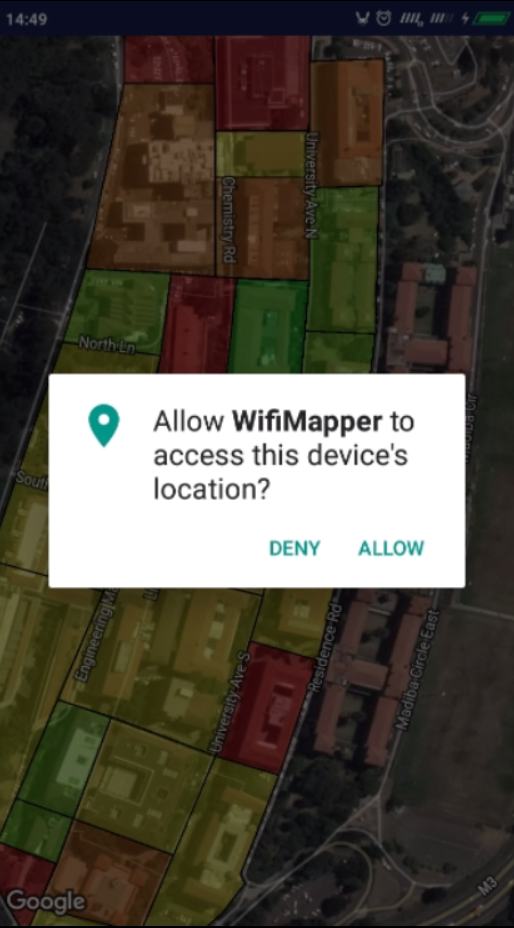
\includegraphics[width=0.7\linewidth]{images_manual/permissions}
	\caption{Asking For Permissions}
	\label{fig:permissions}
\end{figure}

\subsubsection {Map}
On opening the app, a hybrid version of google maps is displayed on the screen. The map contains polygons on top of different buildings with colors depicting the wifi strength on respective WLAN ZONEs. The map is by default zoomed such that it is focused on the University Of Cape Town(UCT) upper campus.

\begin{figure}
	\centering
	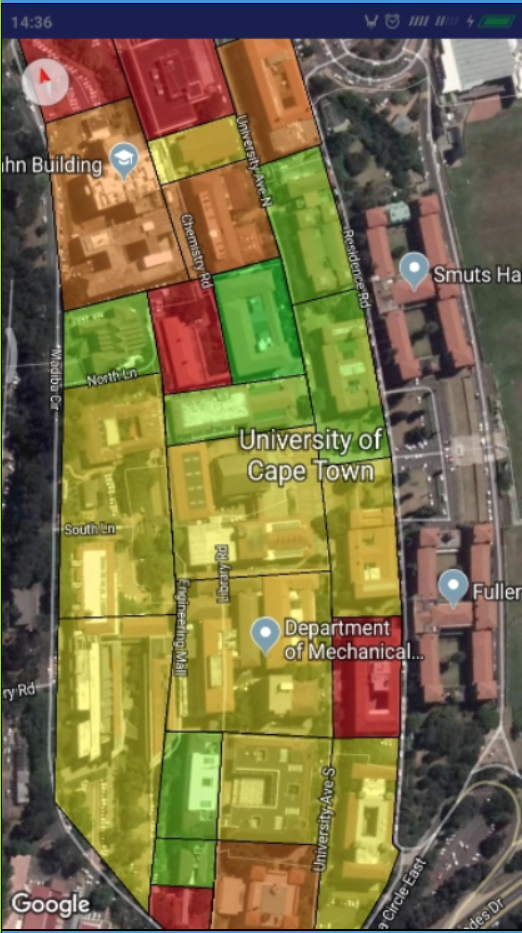
\includegraphics[width=0.7\linewidth]{images_manual/map}
	\caption{Showing the Map}
	\label{fig:map}
\end{figure}

\subsubsection {Zoom}
Wifi mapper allows users to zoomin and zoomout on the map. The app puts restrictions on the zoomout functionality so that the map is always focused at UCT upper campus. The zoomin functionality is also limited to a certain degree. To zoom in, pinch in with two fingers on the map screen. On zooming in the map replaces colored polygons with coloured data points. Zoomout by pinching out on the map screen,if the map was displaying datapoints it replaces those with coloured polygons.
\begin{figure}
	\centering
	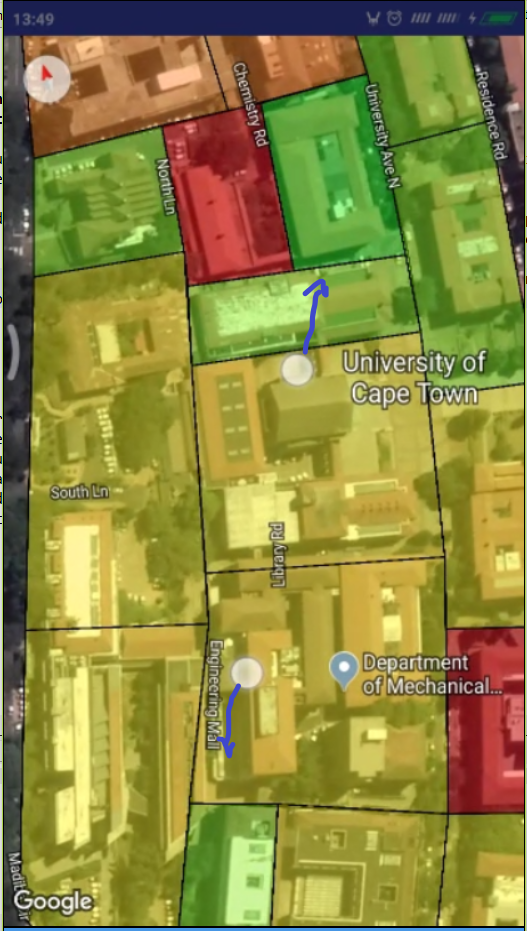
\includegraphics[width=0.7\linewidth]{images_manual/zoomin}
	\caption{zoomin}
	\label{fig:zoomin}
\end{figure}

\begin{figure}
	\centering
	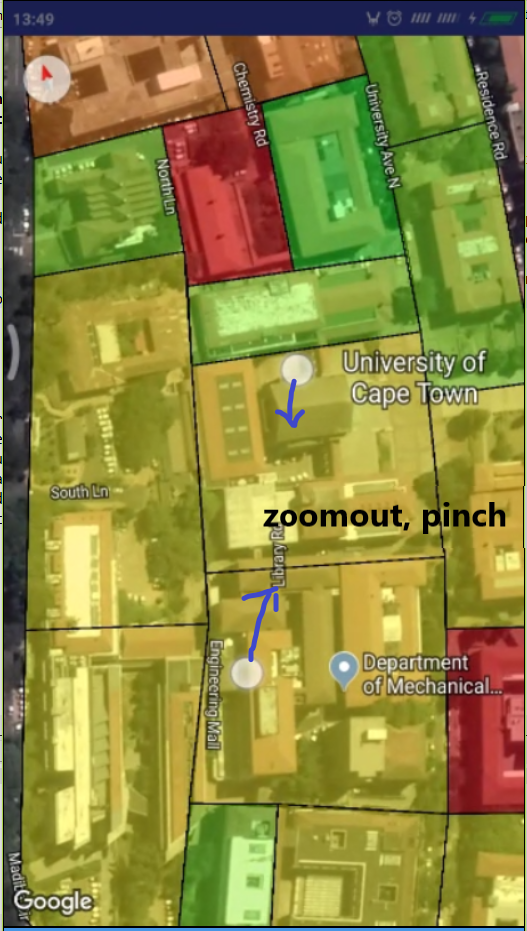
\includegraphics[width=0.7\linewidth]{images_manual/zoomout}
	\caption{zoomout}
	\label{fig:zoomout}
\end{figure}


\subsubsection{Pan}
To move to another area without zooming in, pan on the screen with a single finger. To move the map to the right push the map with a single finger to the left. To move the map to the left push on the map right using a single finger. Rate at which you push the map determines the rate at which the map moves in the specified direction.
\begin{figure}
	\centering
	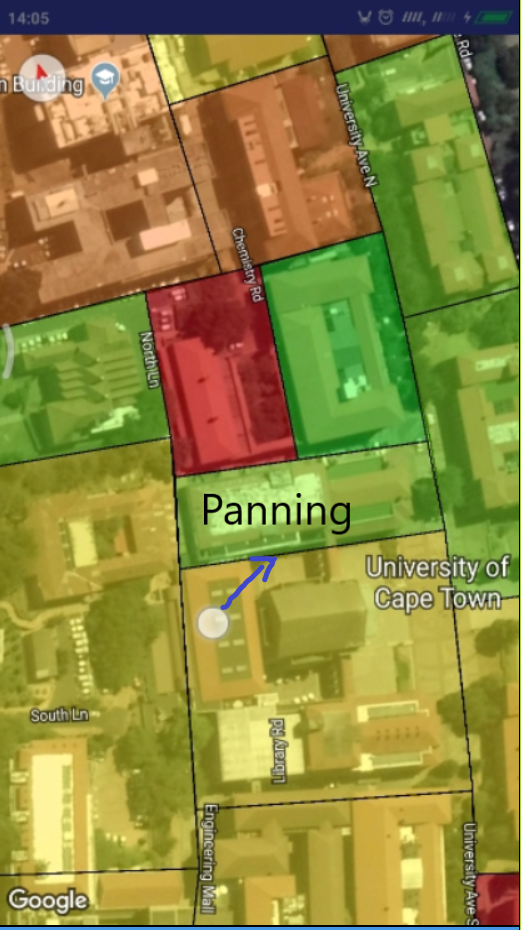
\includegraphics[width=0.7\linewidth]{images_manual/panning}
	\caption{Panning}
	\label{fig:panning}
\end{figure}


\subsubsection{Area tap}
To get the name and wifi strength of an area a polygon is placed over, tap the screen once. On taping the screen the maps pans over to the tapped polygon or area.
\begin{figure}
	\centering
	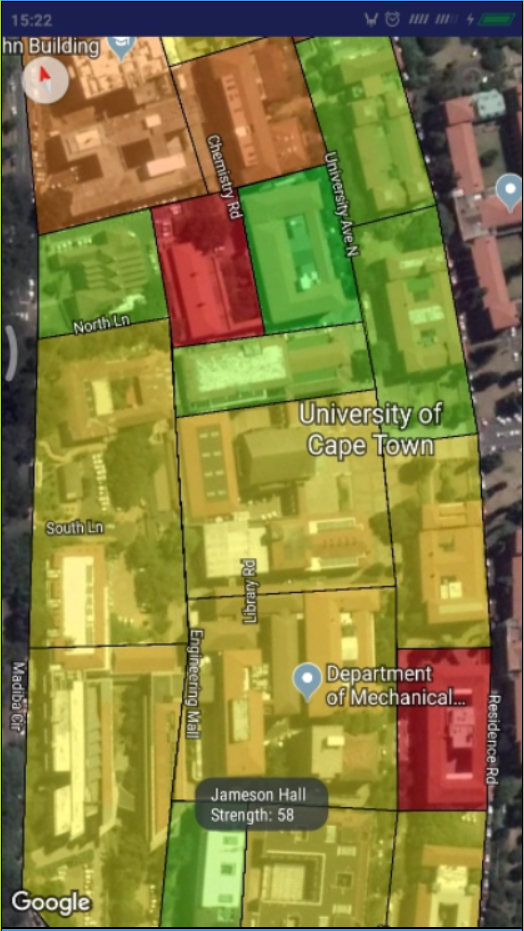
\includegraphics[width=0.7\linewidth]{images_manual/tap}
	\caption{Tapping showing the name and strength of the tapped WLAN ZONE}
	\label{fig:tap}
\end{figure}


\subsection{Web Client}
\subsubsection{Getting started and Installation}
To get started with the web client, open your browser and go to
https://capestone-a8a58.firebaseapp.com/. Before going to the url first ensure that you are connected to the internet. If the network is slow, wait for the app to load fully.

\subsubsection {Map}
On opening the app, a hybrid version of google maps is displayed on the screen. The map contains polygons on top of different buildings with colors depicting the wifi strength on respective WLAN ZONEs. The map is by default zoomed such that it is focused on the University Of Cape Town(UCT) upper campus.

\begin{figure}
	\centering
	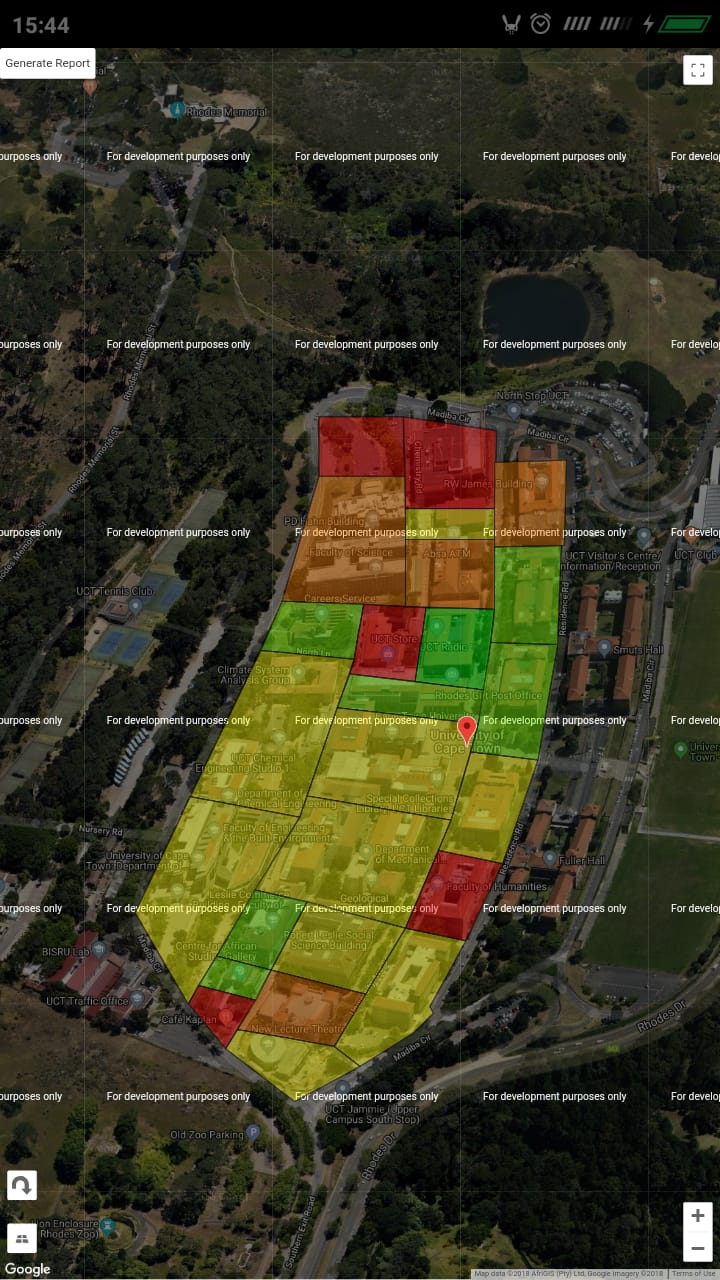
\includegraphics[width=0.7\linewidth]{images_manual/web_map}
	\caption{web client map}
	\label{fig:webmap}
\end{figure}


\subsubsection {Zoom}
Wifi mapper web client allows users to zoomin and zoomout on the map. The app puts restrictions on the zoomout functionality so that the map is always focused at UCT upper campus. The zoomin functionality is also limited to a certain degree. To zoom in, pinch in with two fingers on the map screen. On zooming in the map replaces colored polygons with coloured data points. Zoomout by pinching out on the map screen,if the map was displaying datapoints it replaces those with coloured polygons. On the webclient the zoomin and zoomout limits are different.

\subsubsection{Pan}
The WiFi mapper web client allows users to pan and navigate the map around. To pan use two fingers to move the map around. To move the map to the left push to the right using both fingers. To move them map to the right push on the map to the left with both fingers.

\subsubsection{Area tap}
The behaviour is the same as that of the android client


\subsubsection{Generate Report}
Wifi mapper web app provides capabilities to generate a report from the collected data. To generate the report, on the map click the Generate Report button at the top left corner of the map view. This will take you to the login page. To login the fill in the form fields and click login. If succesful you will be redirected to the report view that contains different charts for the data obtained from the database. On the report view you can interact by hovering over each element of the charts provided to get supplementary data of the chart.

\begin{figure}
	\centering
	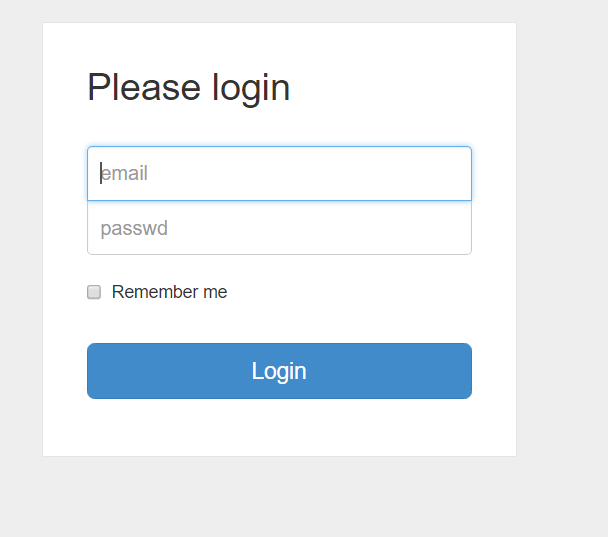
\includegraphics[width=0.7\linewidth]{images_manual/login}
	\caption{login page}
	\label{fig:login}
\end{figure}

\begin{figure}
	\centering
	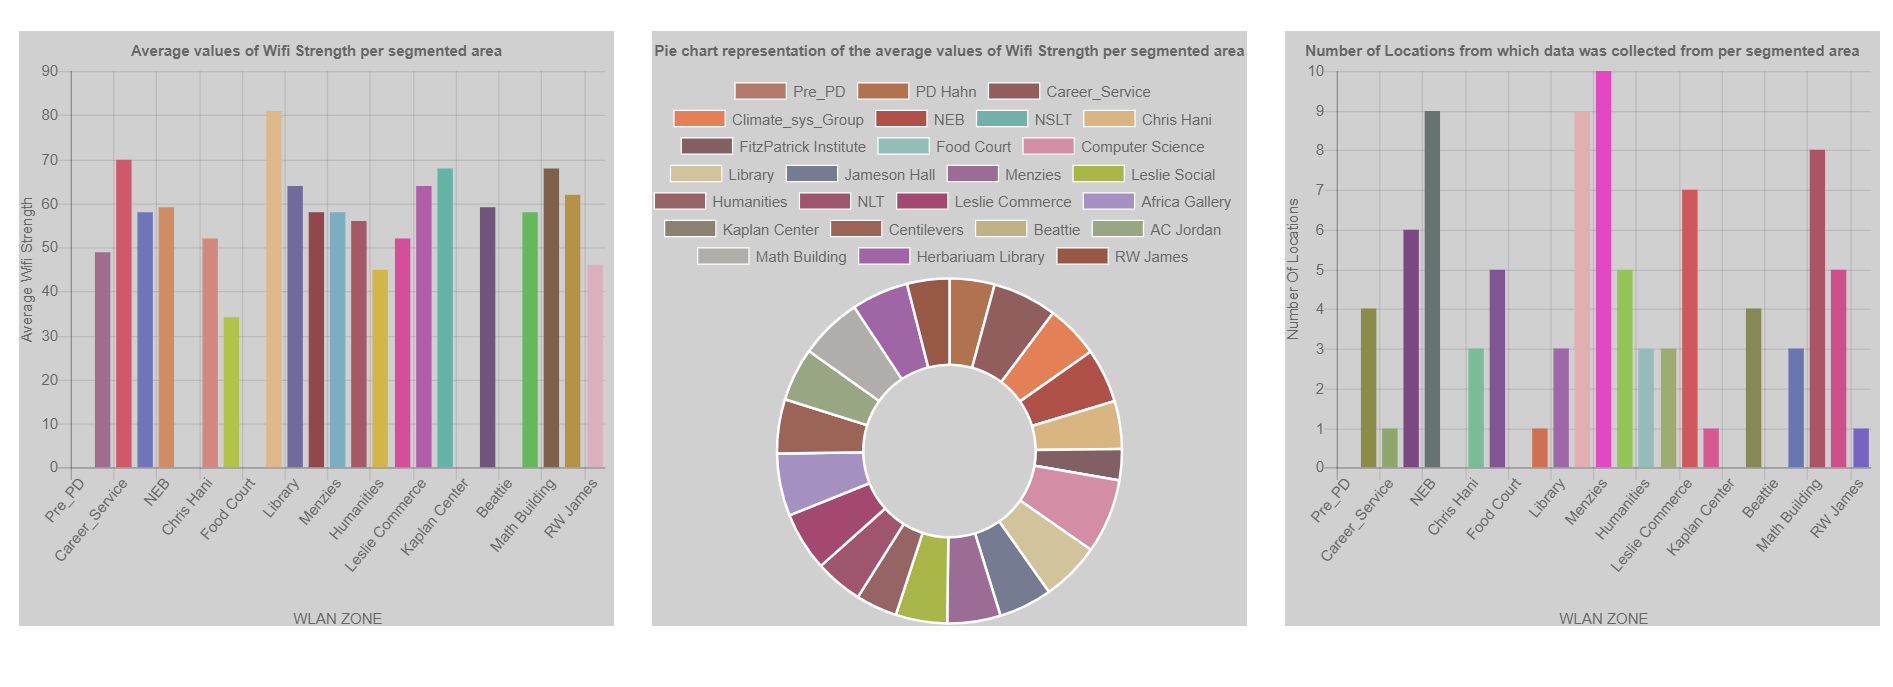
\includegraphics[width=0.7\linewidth]{images_manual/report}
	\caption{a part of the report page}
	\label{fig:report}
\end{figure}


Your system must have a user manual. Append this to your report (make
it Appendix A) or bind it separately if it is big. If your system is
interactive and has a good user interface with context dependent help
then this can be just a cheat sheet. Discuss the level at which your
user manual is to be pitched with your client. If your system is to be
extended then you might want to include a technical API manual.

